% !TeX spellcheck = en_GB
\ifcsname SlidesDistr\endcsname%
\documentclass[handout,aspectratio=169]{beamer}
\else%
\documentclass[aspectratio=169]{beamer}
\fi%
\usepackage{fontspec}
\usepackage[T1]{fontenc}
\usepackage{amsmath}
\usepackage{amsfonts}
\usepackage{amssymb}
\usepackage{graphicx}
\usepackage{csquotes}
\usepackage{booktabs}
\usepackage{multicol}
\usepackage{enumerate}
\usepackage{microtype}
\usepackage[labelfont=bf,font={small}]{caption}
\usepackage{hyperref}
\usepackage{booktabs}
\usepackage{subcaption}
\usepackage{fancyhdr}
\usepackage{pdfpages}
\usepackage{siunitx}
\usepackage{tikz}
\usepackage{mdframed}

\defaultfontfeatures{Mapping=tex-text}
\newfontfamily\symbolfont{Symbola}
\newfontfamily\quotefont{Gentium}

\usepackage[sorting=none]{biblatex}
\addbibresource{../bibliography.bib}

\author{Andreas Stöckel}


\renewcommand{\vec}[1]{{\mathbf{#1}}}
\newcommand{\mat}[1]{{\mathbf{#1}}}
\newcommand{\T}{\ensuremath{\mathsf{T}}}
\renewcommand{\epsilon}{\varepsilon}
\renewcommand{\phi}{\varphi}

% Tango color palette
\definecolor{butter1}{HTML}{FCE94F}
\definecolor{butter2}{HTML}{EDD400}
\definecolor{butter3}{HTML}{C4A000}
\definecolor{orange1}{HTML}{FCAF3E}
\definecolor{orange2}{HTML}{F57900}
\definecolor{orange3}{HTML}{CE5C00}
\definecolor{chocolate1}{HTML}{E9B96E}
\definecolor{chocolate2}{HTML}{C17D11}
\definecolor{chocolate3}{HTML}{8F5902}
\definecolor{chameleon1}{HTML}{8AE234}
\definecolor{chameleon2}{HTML}{73D216}
\definecolor{chameleon3}{HTML}{4E9A06}
\definecolor{skyblue1}{HTML}{729FCF}
\definecolor{skyblue2}{HTML}{3465A4}
\definecolor{skyblue3}{HTML}{204A87}
\definecolor{plum1}{HTML}{AD7FA8}
\definecolor{plum2}{HTML}{75507B}
\definecolor{plum3}{HTML}{5C3566}
\definecolor{scarletred1}{HTML}{EF2929}
\definecolor{scarletred2}{HTML}{CC0000}
\definecolor{scarletred3}{HTML}{A40000}
\definecolor{aluminium1}{HTML}{EEEEEC}
\definecolor{aluminium2}{HTML}{D3D7CF}
\definecolor{aluminium3}{HTML}{BABDB6}
\definecolor{aluminium4}{HTML}{888A85}
\definecolor{aluminium5}{HTML}{555753}
\definecolor{aluminium6}{HTML}{2E3436}

\definecolor{violet}{HTML}{AA305C}
\definecolor{uwyellow}{HTML}{FDD433}
\definecolor{background}{HTML}{F9F9F6}
\definecolor{text}{HTML}{000000}

\definecolor{uweng1}{HTML}{D1B2EE}
\definecolor{uweng2}{HTML}{BF33DE}
\definecolor{uweng3}{HTML}{8001B3}
\definecolor{uweng4}{HTML}{56048A}

\setbeamercolor{title}{fg=violet}
\setbeamercolor{frametitle}{fg=black}
\setbeamercolor{structure}{fg=aluminium5}
\setbeamercolor{normal text}{fg=text}

\setbeamertemplate{navigation symbols}{}
\setbeamertemplate{footline}[frame number]

\hypersetup{%
	colorlinks=false,% hyperlinks will be black
	urlbordercolor=aluminium4,% hyperlink borders will be red
	pdfborderstyle={/S/U/W 0.5}% border style will be underline of width 1pt
}

\makeatletter
\newcommand{\superimpose}[2]{%
	{\ooalign{{#1}\hidewidth\cr{#2}\hidewidth\cr}}}
\makeatother
\newcommand{\SolidCircle}[2]{\superimpose{\color{#1}\symbolfont ⬤}{\textbf{\color{white}#2}}\hspace{1em}}
\newcommand{\OPlus}{\SolidCircle{chameleon3}{\kern0.75pt+}}
\newcommand{\OMeh}{\SolidCircle{uwyellow}{~}}
\newcommand{\OMinus}{\SolidCircle{scarletred3}{\kern2.25pt--}}

\newcommand{\hl}[1]{\colorbox{uwyellow}{{\color{black}\textbf{#1}}}}

\newcommand{\ImageSources}[1]{%
	\begin{columns}%
		\column{1.1\textwidth}%
		\raggedright%
		\tiny\color{aluminium4}%
		\setlength\lineskip{1em}%
		\textbf{Image Sources.}	{#1}%
	\end{columns}}

\newcommand{\ColorRect}[3]{{\color{#1}\rule{#2}{#3}}}
\setbeamertemplate{headline}{\ColorRect{black}{\textwidth}{4pt}\newline\ColorRect{uweng1}{0.25\textwidth}{4pt}\ColorRect{uweng2}{0.25\textwidth}{4pt}\ColorRect{uweng3}{0.25\textwidth}{4pt}\ColorRect{uweng4}{0.25\textwidth}{4pt}}

\newcommand{\MakeTitle}{%
	\vspace{0.5cm}%
	{\textbf{\inserttitle}}\\[0.5cm]%
	\insertauthor\\[0.5cm]%
	\insertdate\\%
	\vspace{2cm}%
 	
\includegraphics[width=7cm]{../assets/uwlogo_eng.pdf}%
}

\newcommand{\handwritingframe}{%
	\begin{frame}
		\begin{columns}
			\column{\paperwidth}
			
\includegraphics{../assets/handwriting_lines.pdf}
		\end{columns}
	\end{frame}	
}

\newcommand{\imageframe}[1]{%
	\setbeamertemplate{navigation symbols}{}%
	\begin{frame}[plain,noframenumbering]%
		\begin{tikzpicture}[remember picture,overlay]%
		\node[at=(current page.center)] {%
			\includegraphics[width=\paperwidth]{#1}%
		};%
		\end{tikzpicture}%
	\end{frame}%
}

\newcommand{\videoframe}[3][mp4]{%
	\begin{frame}[plain,noframenumbering]%
		\hypersetup{%
			pdfborderstyle={/S/U/W 0}% border style will be underline of width 1pt
		}%
		\begin{tikzpicture}[remember picture,overlay]%
		\node[at=(current page.center)] {%
			\includegraphics[width=\paperwidth]{{{video/#2_#3}.jpg}}%
		};%
		\node[at=(current page.center)] {%
			\ifcsname SlidesDistr\endcsname%
				\href{https://youtu.be/#3}{
\includegraphics[width=2cm]{../assets/play_button.pdf}}%
			\else%
				\href{video/#2_#3.#1}{
\includegraphics[width=2cm]{../assets/play_button.pdf}}%
			\fi%
		};%
		\end{tikzpicture}%
	\end{frame}%
}

\newcommand{\includevideo}[4][mp4]{%
	\begingroup%
	\hypersetup{%
		pdfborderstyle={/S/U/W 0}% border style will be underline of width 1pt
	}%
	\begin{tikzpicture}%
	\node (A) {%
		\includegraphics[width=#4]{{{video/#2_#3}.jpg}}%
	};%
	\node[at=(A.center)] {%
		\ifcsname SlidesDistr\endcsname%
			\href{https://youtu.be/#3}{
\includegraphics[width=2cm]{../assets/play_button.pdf}}%
		\else%
			\href{video/#2_#3.#1}{
\includegraphics[width=2cm]{../assets/play_button.pdf}}%
		\fi%
	};%
	\end{tikzpicture}%
	\endgroup%
}

\newcommand{\backupbegin}{
	\newcounter{finalframe}
	\setcounter{finalframe}{\value{framenumber}}
	\setbeamertemplate{footline}{}
}

\newcommand{\backupend}{
	\setcounter{framenumber}{\value{finalframe}}
}


\usepackage{ragged2e}

\newcommand{\Pred}[1]{\mathbf{\textcolor{scarletred3}{#1}}}
\newcommand{\Obj}[1]{\mathtt{\textcolor{skyblue3}{#1}}}
\newcommand{\Fun}[1]{\mathit{\textcolor{chameleon3}{#1}}}
\newcommand{\CC}{\circledast}

\date{March 10 \& 12, 2020\\[-1cm]~~}
\title{SYDE 556/750 \\ Simulating Neurobiological Systems \\ Lecture 10: Symbols and Symbol-like Representations}

\begin{document}
	
	\begin{frame}{}
		\vspace{0.5cm}
		\begin{columns}[c]
			\column{0.6\textwidth}
			\MakeTitle
			\column{0.4\textwidth}
			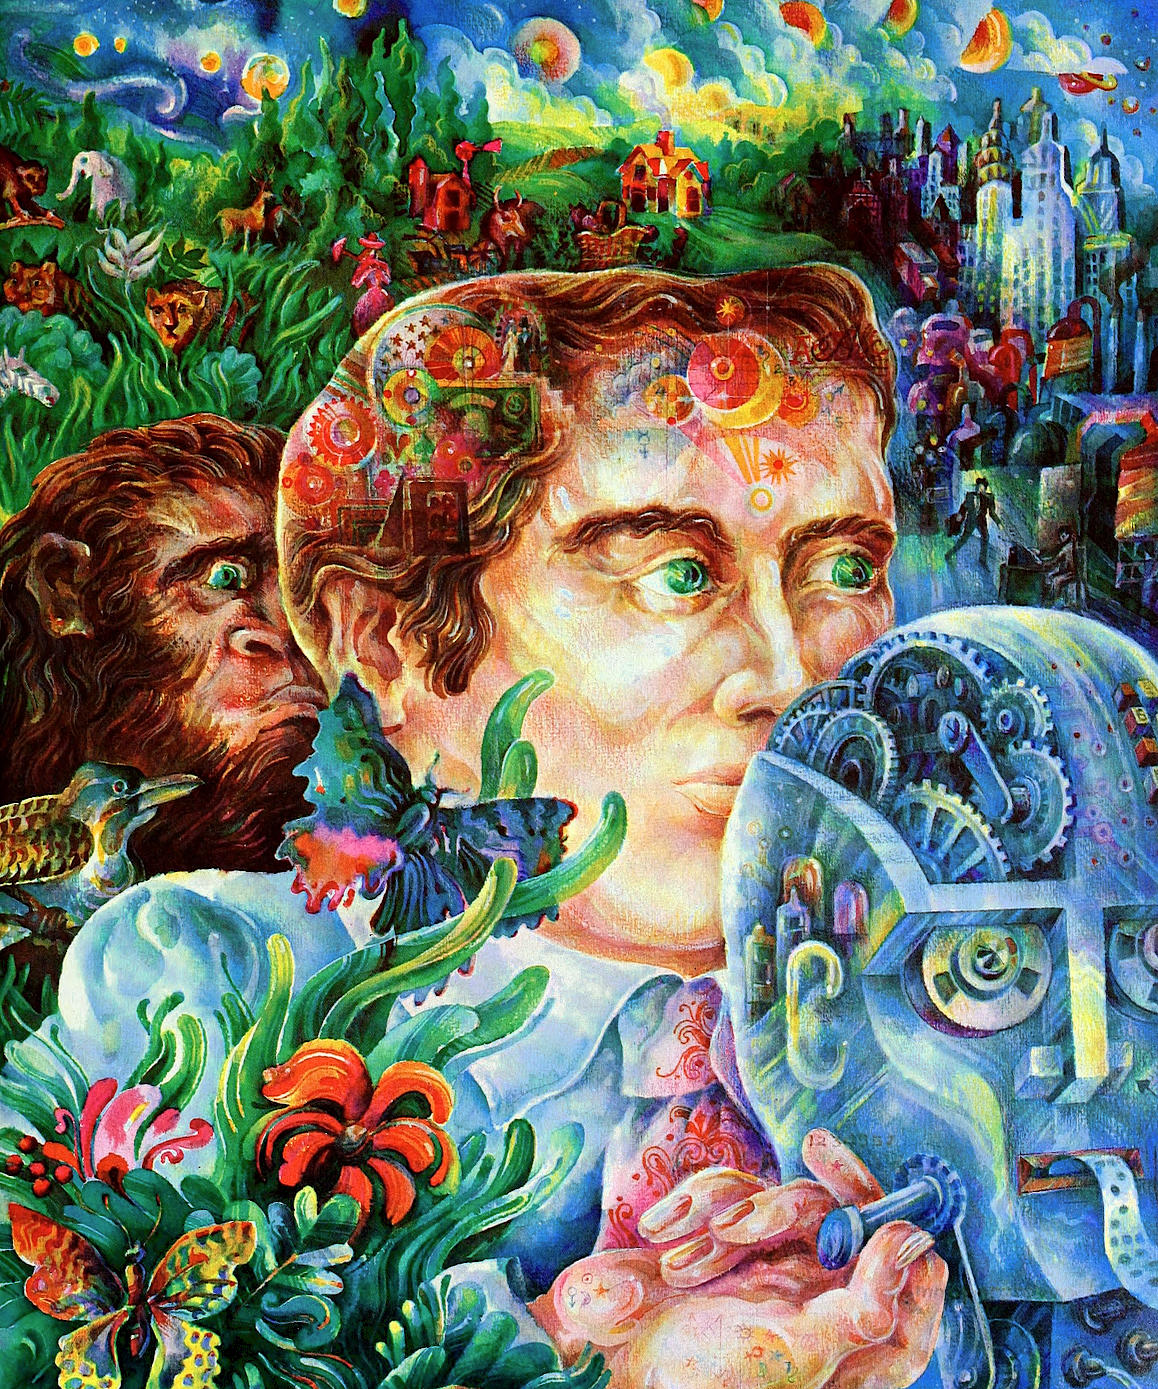
\includegraphics[width=\textwidth]{media/bell_telephone_magazine_1922_14733423296_small_2.jpg}
		\end{columns}
	\end{frame}

	\begin{frame}{Classical Representation of Knowledge}
		\begin{itemize}
			\item \enquote{The number eight comes after the number nine}: $$\Pred{isSucc}(\Obj{EIGHT}, \Obj{NINE})\,.$$
			\item \enquote{All dogs chase cats}: $$\forall x \forall y \, \big ( \Pred{isDog}(x) \wedge \Pred{isCat}(y) \big) \rightarrow \Pred{doesChase}(x, y)\,.$$
			\item \enquote{Anne knows that Bill thinks that Charlie likes Dave}:$$\Pred{knows}\Big(\Obj{ANNE}, ``\Pred{thinks}\big(\Obj{BILL}, `\Pred{likes}(\Obj{CHARLIE}, \Obj{DAVE})\text{'}\big)\text{''}\Big)\,.$$
		\end{itemize}
	\end{frame}

	\begin{frame}{Solution Attempt 1: Neural Synchrony (I)}
		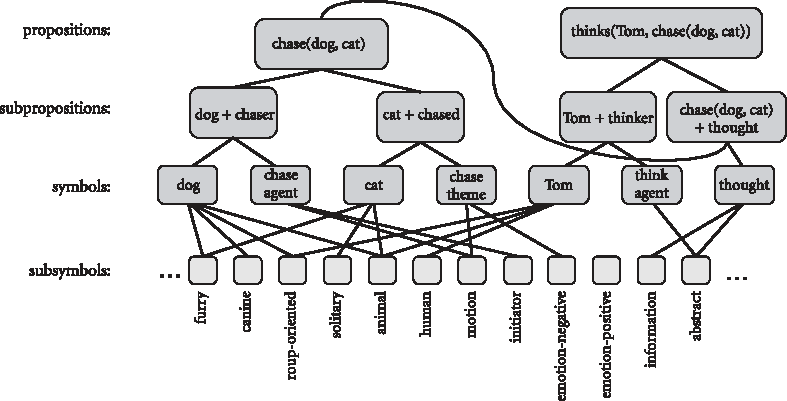
\includegraphics[width=\textwidth]{media/eliasmith_2013_lisa.pdf}
	\end{frame}

	\begin{frame}{Solution Attempt 1: Neural Synchrony (II)}
		\begin{multicols}{2}
			\begin{itemize}
				\setlength{\itemsep}{0.33cm}
				\item[\OPlus] Solves the binding problem
				\item[\OMeh] Localist representation
				\item[\OMeh] Unclear how to solve problems 1 to 3
				\columnbreak
				\item[\OMinus] Unclear how these oscillations are generated and controlled
				\item[\OMinus] Unclear how the representations are processed
				\item[\OMinus] Exponential explosion of neurons required to represent concepts
			\end{itemize}
		\end{multicols}
	\end{frame}

	\begin{frame}{Solution Attempt 2: Neural Blackboard Architecture (I)}
		\centering
		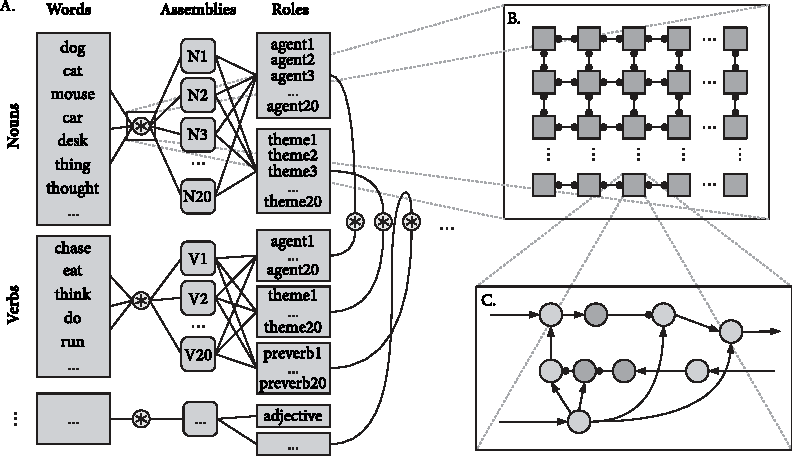
\includegraphics[height=7.25cm]{media/eliasmith_2013_blackboard.pdf}
	\end{frame}

	\begin{frame}{Solution Attempt 2: Neural Blackboard Architecture (II)}
		\centering
		\begin{multicols}{2}
			\begin{itemize}
				\setlength{\itemsep}{0.33cm}
				\item[\OPlus] Fewer resources than LISA
				\item[\OPlus] Solves all four of Jackendoffs challenges (according to the authors)
				\item[\OPlus] Explains limitations of human sentence representation
				\item[\OMeh] (At least partially) localist representation
				\columnbreak
				\item[\OMinus] Particular structure; does not match biology
				\item[\OMinus] Large number of neurons; about $500\times 10^6$ to represent sentences
				\item[\OMinus] Only considers \emph{representation},\\no control structures
			\end{itemize}
		\end{multicols}
	\end{frame}

	\begin{frame}{Solution Attempt 3: Vector Operators}
		\centering
		\textbf{Idea:}  High-dimensional vectors $\vec x \in \mathbb{R}^d$ represent symbols; bind using tensor product\\\vspace*{-0.33cm}
		\small
		\begin{align*}
		\begin{pmatrix}a_1\\a_2\\a_3\end{pmatrix} \otimes \begin{pmatrix}b_1\\b_2\\b_3\end{pmatrix} &=
		\begin{pmatrix}
		a_1 b_1 & a_1 b_2 & a_1 b_3 \\
		a_2 b_1 & a_2 b_2 & a_2 b_3 \\
		a_3 b_1 & a_3 b_2 & a_3 b_3
		\end{pmatrix} && \text{(Outer product)} \\[0.25cm]
		\begin{pmatrix}a_{11} & a_{12} \\ a_{21} & a_{22} \end{pmatrix} \otimes
		\begin{pmatrix}b_{11} & b_{12} \\ b_{21} & b_{22} \end{pmatrix} &=
		\begin{pmatrix}
		a_{11} \begin{pmatrix}b_{11} & b_{12} \\ b_{21} & b_{22} \end{pmatrix} &
		a_{12} \begin{pmatrix}b_{11} & b_{12} \\ b_{21} & b_{22} \end{pmatrix} \\
		a_{21} \begin{pmatrix}b_{11} & b_{12} \\ b_{21} & b_{22} \end{pmatrix} &
		a_{22} \begin{pmatrix}b_{11} & b_{12} \\ b_{21} & b_{22} \end{pmatrix}
		\end{pmatrix} && \text{(Tensor product)}\\ &= 
		\begin{pmatrix}
		a_{11} b_{11} & a_{11} b_{12} & a_{12} b_{11} & a_{12} b_{12} \\
		a_{11} b_{21} & a_{11} b_{22} & a_{12} b_{21} & a_{12} b_{22} \\
		a_{21} b_{11} & a_{21} b_{12} & a_{22} b_{11} & a_{22} b_{12} \\
		a_{21} b_{21} & a_{21} b_{22} & a_{22} b_{21} & a_{22} b_{22}
		\end{pmatrix}
		\end{align*}
		\vspace*{-0.25cm}
		\begin{itemize}
			\centering
			\item<2->[\OMinus] Scales extremely poorly $d^n$ for $n$ binding operations
		\end{itemize}
	\end{frame}

	\begin{frame}{A Deeper Problem: Cognitive Science vs. Neuroscience}
		\begin{columns}
		\column{0.63\textwidth}
		\begin{itemize}
			\setlength{\itemsep}{0.75cm}
			\item Trying very hard to map purely symbolic architectures onto neurons.
			\item Neural aspects are treated as\\\emph{mere implementation details}.
			\item Instance of \hl{top-down modelling}:\\High-level cognitive architectures are mapped onto biology.
			\item Hope of many cognitive scientists:\\If successful, \hl{neurons do not matter}.
		\end{itemize}
		\column{0.37\textwidth}
		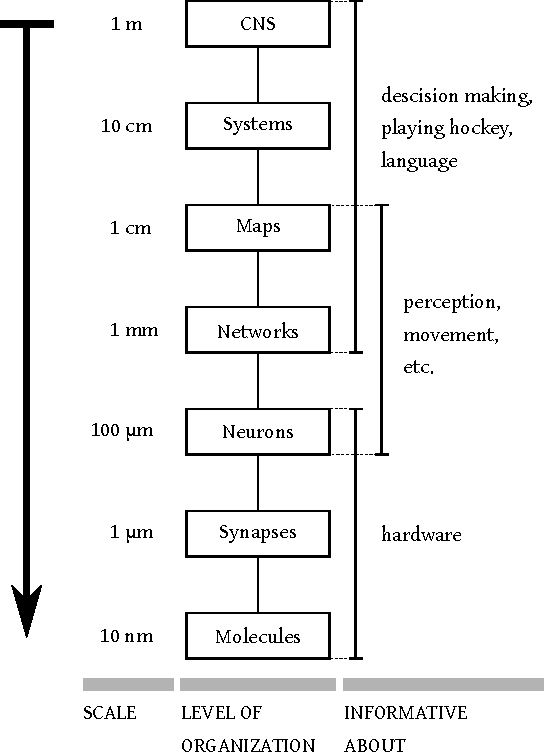
\includegraphics[width=\textwidth]{media/levels_direction_top_down.pdf}
		\end{columns}
	\end{frame}

	\begin{frame}{VSAs: Potential Binding Operators (I)}
		\begin{align*}
		\begin{pmatrix}1 \\ 0 \\ 1 \\ 0\end{pmatrix} \oplus \begin{pmatrix}1 \\ 1 \\ 0 \\ 0\end{pmatrix} &= \begin{pmatrix}0 \\ 1 \\ 1 \\ 0\end{pmatrix} && \textit{(XOR)}\\
		\begin{pmatrix}A \\ B \\ C \\ D\end{pmatrix} \odot \begin{pmatrix}E \\ F \\ G \\ H\end{pmatrix} &= \begin{pmatrix}AE \\ BF \\ CG \\ DH\end{pmatrix} && \textit{(Hadamard Product)}
		\end{align*}
	\end{frame}

	\begin{frame}{VSAs: Potential Binding Operators (II)}
		\begin{align*}
		\begin{pmatrix}A \\ B \\ C \\ D\end{pmatrix} \CC \begin{pmatrix}E \\ F \\ G \\ H\end{pmatrix} &= \begin{pmatrix}AE &+& BH &+& CG &+& DF \\ AF &+& BE &+& CH &+& DG \\ AG &+& BF &+& CE &+& DH \\ AH &+& BG &+& CF &+& DE\end{pmatrix} && \textit{(Circular Convolution)}
		\end{align*}
		\vspace{0.25cm}
		Circular Convolution is a \enquote{compressed} outer product:\\[0.25cm]
		\hspace{0.7cm}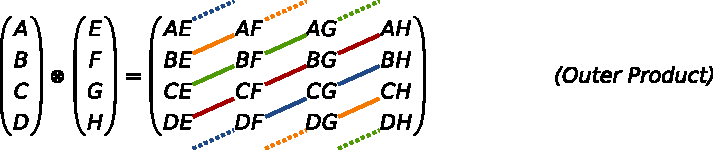
\includegraphics{media/cconv_outer_product.pdf}
	\end{frame}

	\begin{frame}{Sentence Encoding Revisited}
		\begin{itemize}
			\item \enquote{The number eight comes after the number nine}:
			\begin{align*}
			\Obj{NUMBER} \CC \Obj{EIGHT} + \Obj{SUCC} \CC \Obj{NINE} \,.
			\end{align*}
			\item \enquote{The dog chases the cat}:
			\begin{align*}
			\Obj{DOG} \CC \Obj{SUBJ} + \Obj{CAT} \CC \Obj{OBJ} + \Obj{CHASE} \CC \Obj{VERB} \,.
			\end{align*}
			\item \enquote{Anne knows that Bill thinks that Charlie likes Dave}:
			\begin{align*}
			\Obj{SUBJ} \CC \Obj{ANNE} + \Obj{ACT} \CC \Obj{KNOWS} + \Obj{OBJ} \CC \\\Big(\Obj{SUBJ} \CC \Obj{BILL} + \Obj{ACT} \CC \Obj{THINKS} + \Obj{OBJ} \CC \\ \big(\Obj{SUBJ} \CC \Obj{CHARLIE} + \Obj{ACT} \CC \Obj{LIKES} + \Obj{OBJ} \CC \Obj{DAVE}\big)\Big) \,.
			\end{align*}
		\end{itemize}
		\vspace{-0.25cm}
		\begin{itemize}
			\centering
			\item<2->[\symbolfont ⚠] \hl{Compression of information; graceful degradation}
		\end{itemize}
	\end{frame}

	\begin{frame}{Circular Convolution: Dissimilarity and Reversibility}
		\centering
		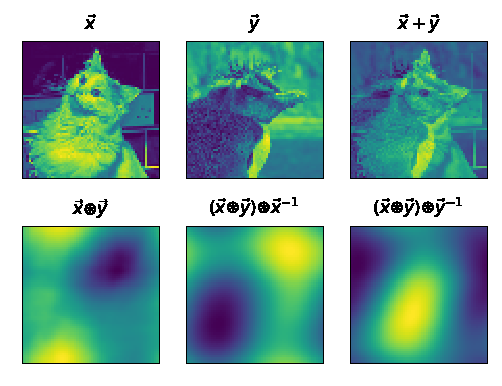
\includegraphics[height=7.25cm]{media/cconv_sim.pdf}
	\end{frame}

	\backupbegin

	\begin{frame}[noframenumbering]{Image sources}
		\small
		\textbf{Title slide}\\Bell telephone magazine, 1922,  American Telephone and Telegraph Company\\ \href{https://commons.wikimedia.org/wiki/File:Bell_telephone_magazine_(1922)_(14733423296).jpg}{Wikimedia}.
	\end{frame}

	\backupend
	
\end{document}
